\documentclass[]{article}
\usepackage{lmodern}
\usepackage{amssymb,amsmath}
\usepackage{ifxetex,ifluatex}
\usepackage{fixltx2e} % provides \textsubscript
\ifnum 0\ifxetex 1\fi\ifluatex 1\fi=0 % if pdftex
  \usepackage[T1]{fontenc}
  \usepackage[utf8]{inputenc}
\else % if luatex or xelatex
  \ifxetex
    \usepackage{mathspec}
  \else
    \usepackage{fontspec}
  \fi
  \defaultfontfeatures{Ligatures=TeX,Scale=MatchLowercase}
\fi
% use upquote if available, for straight quotes in verbatim environments
\IfFileExists{upquote.sty}{\usepackage{upquote}}{}
% use microtype if available
\IfFileExists{microtype.sty}{%
\usepackage{microtype}
\UseMicrotypeSet[protrusion]{basicmath} % disable protrusion for tt fonts
}{}
\usepackage[margin=1in]{geometry}
\usepackage{hyperref}
\hypersetup{unicode=true,
            pdftitle={Effect of Vitamin C on Tooth Growth of Guinea pigs},
            pdfauthor={Tomás A. Maccor},
            pdfborder={0 0 0},
            breaklinks=true}
\urlstyle{same}  % don't use monospace font for urls
\usepackage{color}
\usepackage{fancyvrb}
\newcommand{\VerbBar}{|}
\newcommand{\VERB}{\Verb[commandchars=\\\{\}]}
\DefineVerbatimEnvironment{Highlighting}{Verbatim}{commandchars=\\\{\}}
% Add ',fontsize=\small' for more characters per line
\usepackage{framed}
\definecolor{shadecolor}{RGB}{248,248,248}
\newenvironment{Shaded}{\begin{snugshade}}{\end{snugshade}}
\newcommand{\AlertTok}[1]{\textcolor[rgb]{0.94,0.16,0.16}{#1}}
\newcommand{\AnnotationTok}[1]{\textcolor[rgb]{0.56,0.35,0.01}{\textbf{\textit{#1}}}}
\newcommand{\AttributeTok}[1]{\textcolor[rgb]{0.77,0.63,0.00}{#1}}
\newcommand{\BaseNTok}[1]{\textcolor[rgb]{0.00,0.00,0.81}{#1}}
\newcommand{\BuiltInTok}[1]{#1}
\newcommand{\CharTok}[1]{\textcolor[rgb]{0.31,0.60,0.02}{#1}}
\newcommand{\CommentTok}[1]{\textcolor[rgb]{0.56,0.35,0.01}{\textit{#1}}}
\newcommand{\CommentVarTok}[1]{\textcolor[rgb]{0.56,0.35,0.01}{\textbf{\textit{#1}}}}
\newcommand{\ConstantTok}[1]{\textcolor[rgb]{0.00,0.00,0.00}{#1}}
\newcommand{\ControlFlowTok}[1]{\textcolor[rgb]{0.13,0.29,0.53}{\textbf{#1}}}
\newcommand{\DataTypeTok}[1]{\textcolor[rgb]{0.13,0.29,0.53}{#1}}
\newcommand{\DecValTok}[1]{\textcolor[rgb]{0.00,0.00,0.81}{#1}}
\newcommand{\DocumentationTok}[1]{\textcolor[rgb]{0.56,0.35,0.01}{\textbf{\textit{#1}}}}
\newcommand{\ErrorTok}[1]{\textcolor[rgb]{0.64,0.00,0.00}{\textbf{#1}}}
\newcommand{\ExtensionTok}[1]{#1}
\newcommand{\FloatTok}[1]{\textcolor[rgb]{0.00,0.00,0.81}{#1}}
\newcommand{\FunctionTok}[1]{\textcolor[rgb]{0.00,0.00,0.00}{#1}}
\newcommand{\ImportTok}[1]{#1}
\newcommand{\InformationTok}[1]{\textcolor[rgb]{0.56,0.35,0.01}{\textbf{\textit{#1}}}}
\newcommand{\KeywordTok}[1]{\textcolor[rgb]{0.13,0.29,0.53}{\textbf{#1}}}
\newcommand{\NormalTok}[1]{#1}
\newcommand{\OperatorTok}[1]{\textcolor[rgb]{0.81,0.36,0.00}{\textbf{#1}}}
\newcommand{\OtherTok}[1]{\textcolor[rgb]{0.56,0.35,0.01}{#1}}
\newcommand{\PreprocessorTok}[1]{\textcolor[rgb]{0.56,0.35,0.01}{\textit{#1}}}
\newcommand{\RegionMarkerTok}[1]{#1}
\newcommand{\SpecialCharTok}[1]{\textcolor[rgb]{0.00,0.00,0.00}{#1}}
\newcommand{\SpecialStringTok}[1]{\textcolor[rgb]{0.31,0.60,0.02}{#1}}
\newcommand{\StringTok}[1]{\textcolor[rgb]{0.31,0.60,0.02}{#1}}
\newcommand{\VariableTok}[1]{\textcolor[rgb]{0.00,0.00,0.00}{#1}}
\newcommand{\VerbatimStringTok}[1]{\textcolor[rgb]{0.31,0.60,0.02}{#1}}
\newcommand{\WarningTok}[1]{\textcolor[rgb]{0.56,0.35,0.01}{\textbf{\textit{#1}}}}
\usepackage{longtable,booktabs}
\usepackage{graphicx,grffile}
\makeatletter
\def\maxwidth{\ifdim\Gin@nat@width>\linewidth\linewidth\else\Gin@nat@width\fi}
\def\maxheight{\ifdim\Gin@nat@height>\textheight\textheight\else\Gin@nat@height\fi}
\makeatother
% Scale images if necessary, so that they will not overflow the page
% margins by default, and it is still possible to overwrite the defaults
% using explicit options in \includegraphics[width, height, ...]{}
\setkeys{Gin}{width=\maxwidth,height=\maxheight,keepaspectratio}
\IfFileExists{parskip.sty}{%
\usepackage{parskip}
}{% else
\setlength{\parindent}{0pt}
\setlength{\parskip}{6pt plus 2pt minus 1pt}
}
\setlength{\emergencystretch}{3em}  % prevent overfull lines
\providecommand{\tightlist}{%
  \setlength{\itemsep}{0pt}\setlength{\parskip}{0pt}}
\setcounter{secnumdepth}{0}
% Redefines (sub)paragraphs to behave more like sections
\ifx\paragraph\undefined\else
\let\oldparagraph\paragraph
\renewcommand{\paragraph}[1]{\oldparagraph{#1}\mbox{}}
\fi
\ifx\subparagraph\undefined\else
\let\oldsubparagraph\subparagraph
\renewcommand{\subparagraph}[1]{\oldsubparagraph{#1}\mbox{}}
\fi

%%% Use protect on footnotes to avoid problems with footnotes in titles
\let\rmarkdownfootnote\footnote%
\def\footnote{\protect\rmarkdownfootnote}

%%% Change title format to be more compact
\usepackage{titling}

% Create subtitle command for use in maketitle
\providecommand{\subtitle}[1]{
  \posttitle{
    \begin{center}\large#1\end{center}
    }
}

\setlength{\droptitle}{-2em}

  \title{Effect of Vitamin C on Tooth Growth of Guinea pigs}
    \pretitle{\vspace{\droptitle}\centering\huge}
  \posttitle{\par}
    \author{Tomás A. Maccor}
    \preauthor{\centering\large\emph}
  \postauthor{\par}
      \predate{\centering\large\emph}
  \postdate{\par}
    \date{22/3/2020}


\begin{document}
\maketitle

\hypertarget{introduction}{%
\subsection{Introduction}\label{introduction}}

This assignment explores whether 3 different doses \& 2 different
delivery methods of Vitamin C have an influence on the tooth lengths of
Guinea pigs. The dataset used is \textbf{ToothGrowth}, which comes with
R as one of its practice/sample datasets.

Each animal received one of 3 doses of vitamin C, by one of 2 delivery
methods: ascorbic acid (VC) versus orange juice (OJ).

This report comprises:

\begin{itemize}
\tightlist
\item
  A basic/descritive statistics summary of our sample data, plus an
  exploratory analysis.
\item
  Use of statistical inference methods so that if any
  effects/conclusions are obtained from the SAMPLE data (contained in
  the ToothGrowth dataset), we can infer that these effects also apply
  to the entire population of Guinea pigs.
\end{itemize}

\hypertarget{summary-of-data-exploratory-analysis}{%
\subsection{Summary of data \& exploratory
analysis}\label{summary-of-data-exploratory-analysis}}

First glimpse of the ToothGrowth dataset:

\begin{verbatim}
## 'data.frame':    60 obs. of  3 variables:
##  $ len : num  4.2 11.5 7.3 5.8 6.4 10 11.2 11.2 5.2 7 ...
##  $ supp: Factor w/ 2 levels "OJ","VC": 2 2 2 2 2 2 2 2 2 2 ...
##  $ dose: num  0.5 0.5 0.5 0.5 0.5 0.5 0.5 0.5 0.5 0.5 ...
\end{verbatim}

\textbf{LEN = length of odontoblast \emph{(the measure of Tooth Growth)}
}. A NUMERIC variable\\
SUPP = delivery method (VC or OJ). FACTOR variable\\
DOSE = Vitamin C dose: 0.5, 1 \& 2 mg/day. NUMERIC variable

~ ~ ~

How many Guinea pigs received which dose, and by which method?:

\begin{Shaded}
\begin{Highlighting}[]
\NormalTok{a <-}\StringTok{ }\NormalTok{ToothGrowth }\OperatorTok\StringTok{ }\KeywordTok{group_by}\NormalTok{(dose, supp) }\OperatorTok\StringTok{ }\KeywordTok{summarise}\NormalTok{(}\DataTypeTok{n =} \KeywordTok{n}\NormalTok{())}
\NormalTok{knitr}\OperatorTok{::}\KeywordTok{kable}\NormalTok{((a), }\DataTypeTok{caption =} \StringTok{"Nr. of observations in each group"}\NormalTok{)}
\end{Highlighting}
\end{Shaded}

\begin{longtable}[]{@{}rlr@{}}
\caption{Nr. of observations in each group}\tabularnewline
\toprule
dose & supp & n\tabularnewline
\midrule
\endfirsthead
\toprule
dose & supp & n\tabularnewline
\midrule
\endhead
0.5 & OJ & 10\tabularnewline
0.5 & VC & 10\tabularnewline
1.0 & OJ & 10\tabularnewline
1.0 & VC & 10\tabularnewline
2.0 & OJ & 10\tabularnewline
2.0 & VC & 10\tabularnewline
\bottomrule
\end{longtable}

So then, 20 pigs received each of the 3 doses ---\textgreater{} 10 via
VC, 10 via OJ.

\break

Let's have a first visualization of the data:

\begin{Shaded}
\begin{Highlighting}[]
\NormalTok{ToothGrowth}\OperatorTok{$}\NormalTok{dose <-}\StringTok{ }\KeywordTok{as.factor}\NormalTok{(ToothGrowth}\OperatorTok{$}\NormalTok{dose)}

\NormalTok{dose_supp_plot <-}\StringTok{ }\KeywordTok{ggplot}\NormalTok{(ToothGrowth, }\KeywordTok{aes}\NormalTok{(}\DataTypeTok{x =}\NormalTok{ dose, }\DataTypeTok{y =}\NormalTok{ len, }\DataTypeTok{fill =}\NormalTok{ supp))}
\NormalTok{dose_supp_plot }\OperatorTok{+}\StringTok{ }\KeywordTok{geom_boxplot}\NormalTok{() }\OperatorTok{+}\StringTok{ }\KeywordTok{xlab}\NormalTok{(}\StringTok{"Vitamin C dose (mg/day)"}\NormalTok{)}
\end{Highlighting}
\end{Shaded}

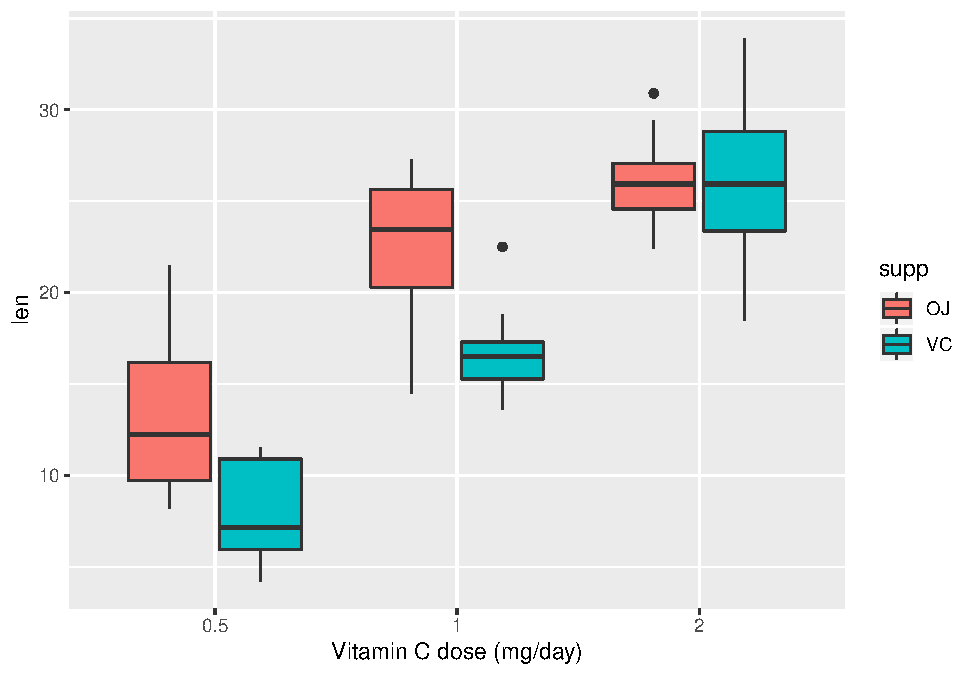
\includegraphics{Statistical-Inference-Assigment---Part-2---Final_files/figure-latex/unnamed-chunk-3-1.pdf}

We can observe what could be a significant difference in Tooth Growth
between the \textbf{0.5 mg/day} dose versus the \textbf{1 \& 2 mg/day}
doses. We need to test for statistical significance to ascertain this.
It would also appear there is a difference between delivering Vitamin C
via \textbf{VC} vs \textbf{OJ} for the \textbf{0.5 \& 1mg/day} doses.

\break

If we plot the tooth growth differences by Vitamin C Dose only, and
obtain the means for the 3 different Vit C doses:

\begin{Shaded}
\begin{Highlighting}[]
\NormalTok{dose_plot <-}\StringTok{ }\KeywordTok{ggplot}\NormalTok{(ToothGrowth, }\KeywordTok{aes}\NormalTok{(}\DataTypeTok{x =}\NormalTok{ dose, }\DataTypeTok{y =}\NormalTok{ len))}
\NormalTok{dose_plot }\OperatorTok{+}\StringTok{ }\KeywordTok{geom_boxplot}\NormalTok{()}
\end{Highlighting}
\end{Shaded}

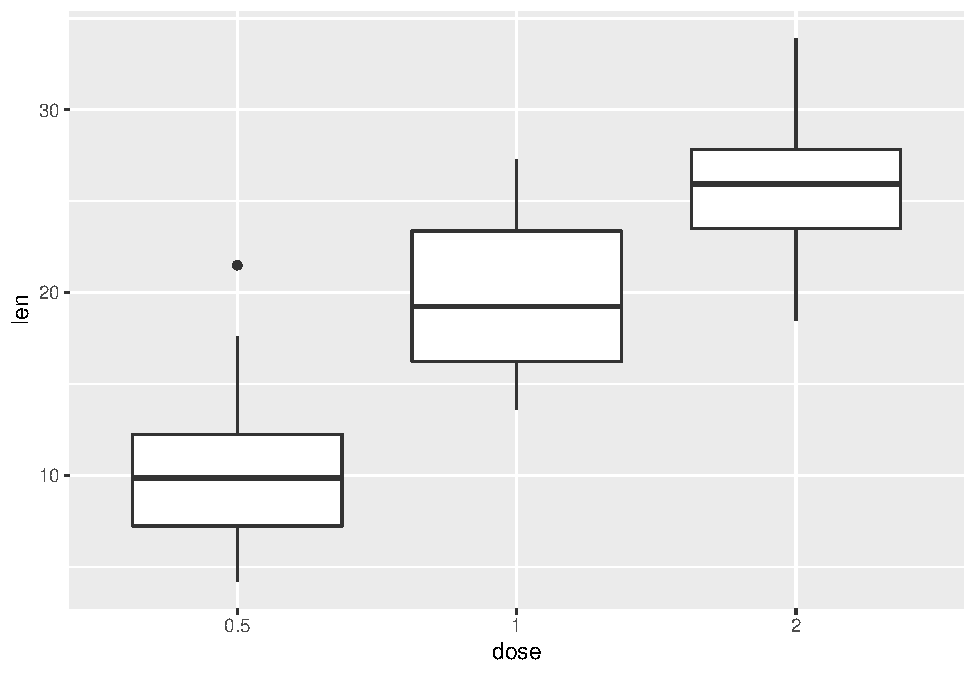
\includegraphics{Statistical-Inference-Assigment---Part-2---Final_files/figure-latex/unnamed-chunk-4-1.pdf}

\begin{Shaded}
\begin{Highlighting}[]
\NormalTok{b <-}\StringTok{ }\NormalTok{ToothGrowth }\OperatorTok\StringTok{ }\KeywordTok{group_by}\NormalTok{(dose) }\OperatorTok\StringTok{ }\KeywordTok{summarise}\NormalTok{(}\DataTypeTok{Mean_Tooth_Growth =} \KeywordTok{mean}\NormalTok{(len))}
\NormalTok{knitr}\OperatorTok{::}\KeywordTok{kable}\NormalTok{(b)}
\end{Highlighting}
\end{Shaded}

\begin{longtable}[]{@{}lr@{}}
\toprule
dose & Mean\_Tooth\_Growth\tabularnewline
\midrule
\endhead
0.5 & 10.605\tabularnewline
1 & 19.735\tabularnewline
2 & 26.100\tabularnewline
\bottomrule
\end{longtable}

This time, it could well be that there's statistical difference between
all 3 doses.

As we have \textgreater{} 2 groups with what appear similar intergroup
variance, we use ANOVA for testing significance (equal variance).

So far, our assumptions are:\\
- That tooth growth in Guinea pigs is normally distributed\\
- That the 3 different DOSE groups have an equal variance

\break

\hypertarget{hypothesis-testing---results---conclusions}{%
\subsection{HYPOTHESIS TESTING - RESULTS -
CONCLUSIONS}\label{hypothesis-testing---results---conclusions}}

\begin{Shaded}
\begin{Highlighting}[]
\NormalTok{ANOVA_dose <-}\StringTok{ }\KeywordTok{aov}\NormalTok{(len }\OperatorTok{~}\StringTok{ }\NormalTok{dose, }\DataTypeTok{data =}\NormalTok{ ToothGrowth)}
\KeywordTok{summary.aov}\NormalTok{(ANOVA_dose)}
\end{Highlighting}
\end{Shaded}

\begin{verbatim}
##             Df Sum Sq Mean Sq F value   Pr(>F)    
## dose         2   2426    1213   67.42 9.53e-16 ***
## Residuals   57   1026      18                     
## ---
## Signif. codes:  0 '***' 0.001 '**' 0.01 '*' 0.05 '.' 0.1 ' ' 1
\end{verbatim}

So, per ANOVA, we have a statistically significant difference in Mean
Tooth Growth between the 3 DOSES (p = 9.53e-16, thus p \textless{}
0.05).

But ANOVA does not allow to know which of the pairwise DOSE comparisons
are significant --we need to perform a TUKEY TEST to determine this:\\
\hspace*{0.333em}\\
\hspace*{0.333em}

\begin{Shaded}
\begin{Highlighting}[]
\KeywordTok{TukeyHSD}\NormalTok{(ANOVA_dose)}
\end{Highlighting}
\end{Shaded}

\begin{verbatim}
##   Tukey multiple comparisons of means
##     95% family-wise confidence level
## 
## Fit: aov(formula = len ~ dose, data = ToothGrowth)
## 
## $dose
##         diff       lwr       upr    p adj
## 1-0.5  9.130  5.901805 12.358195 0.00e+00
## 2-0.5 15.495 12.266805 18.723195 0.00e+00
## 2-1    6.365  3.136805  9.593195 4.25e-05
\end{verbatim}

Which also results in statistically significant differences between all
3 doses (p \textless{} 0.05).\\
The \textbf{differences between the mean DOSES} and the
\textbf{confidence intervals \emph{for those mean differences} } are
listed(provided) in the Tukey Test.

So for example, we can state that if the entire population of Guinea
pigs was given Vitamin C at 3 doses, and we took random samples of these
pigs, 95\% of the times we would obtain a Mean difference in Tooth
Growth that would be between 5.90 to 12.36 (in the 0.5 mg vs.~1.0 mg/day
Vitamin C groups).

\break

~

In relation to the TYPE of Vitamin C delivery method (\textbf{supp}, VC
vs.~OC), we must perform a t-test between the 30 pigs that received
Vitamin C VC versus the 30 that received OJ:

\begin{Shaded}
\begin{Highlighting}[]
\KeywordTok{t.test}\NormalTok{(len }\OperatorTok{~}\StringTok{ }\NormalTok{supp, }\DataTypeTok{data =}\NormalTok{ ToothGrowth)}
\end{Highlighting}
\end{Shaded}

\begin{verbatim}
## 
##  Welch Two Sample t-test
## 
## data:  len by supp
## t = 1.9153, df = 55.309, p-value = 0.06063
## alternative hypothesis: true difference in means is not equal to 0
## 95 percent confidence interval:
##  -0.1710156  7.5710156
## sample estimates:
## mean in group OJ mean in group VC 
##         20.66333         16.96333
\end{verbatim}

The results show that \textbf{there is no statistically significant
difference in Tooth Growth depending on the Vitamin C delivery method
used} (p = 0.06). We can also confirm this result by noting that the
95\% confidence interval for the \emph{difference in means} includes
``0'' as one of the possible values (so, one of the statistically
possible values would be that the Mean(VC) - Mean(OJ) = 0) ~

If we were to perform paired t-tests for VC/OJ, within each of the dose
groups, the result would be similar, with the difference that we would
loose statistical confidence (we would obtain a confidence interval of
85\% at a maximum, which is less certainty, thus is not desired)


\end{document}
